% 半角 引入：正方形 ABCD 边4，E∈BC, F∈CD, ∠EAF=45°，求证 EF=BE+DF
\documentclass[tikz,border=4pt]{standalone}
\usepackage{ctex}
\usepackage{amsmath}
\usetikzlibrary{calc}
\begin{document}
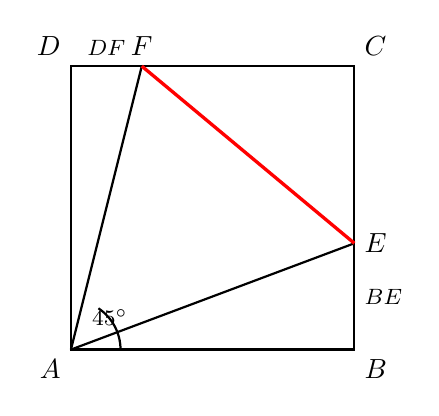
\begin{tikzpicture}[scale=0.9, thick]
  \coordinate (A) at (0,0);
  \coordinate (B) at (4,0);
  \coordinate (C) at (4,4);
  \coordinate (D) at (0,4);
  \coordinate (E) at (4,1.5);
  \coordinate (F) at (1,4);
  \draw (A)--(B)--(C)--(D)--cycle;
  \draw (A)--(E);
  \draw (A)--(F);
  \draw[red, very thick] (E)--(F);
  % 标记 BE 与 DF
  \node[right] at ($(B)!0.5!(E)$) {\footnotesize $BE$};
  \node[above] at ($(D)!0.5!(F)$) {\footnotesize $DF$};
  % 角 45°
  \draw (0.7,0) arc[start angle=0, end angle=56.31, radius=0.7];
  \node at (0.55,0.45) {\footnotesize $45^\circ$};
  \node[below left] at (A) {$A$};
  \node[below right] at (B) {$B$};
  \node[above right] at (C) {$C$};
  \node[above left] at (D) {$D$};
  \node[right] at (E) {$E$};
  \node[above] at (F) {$F$};
\end{tikzpicture}
\end{document}
